% Primarily this section should be about scientific methods and theories you need to evaluate/compare/invent to solve your problems from 1.3.
% In some cases it may be ok to describe different technologies, but the purpose is to describe something and then draw a conclusion from that.
% Example, if you decide to discuss different databases, it may be for the purpose of selecting the best type for your implementation later on (based on for example data representation, scalability, speed, etc.).
% Optimally the problems in 1.3 are not solved by anyone else yet, in which case this section needs to describe how to solve them (new algorithms, mathematical approaches, etc.).
 
% This section can have a lot of subsections (3.1, 3.2, 3.3, etc).

% TODO: Explain what this section will contain.

% TODO: Explain DWARF Sections
The \emph{DWARF} format is divided into sections in the object file which all contain specific information, these sections use offsets to point to information in another section, see figure \ref{fig:dwarfsections}.
All of the sections can be different from depending on \emph{DWARF} versions and some doesn't exist in the older versions.
Thus these explanations only apply to \emph{DWARF} version $4$ and some of the older versions, checkout Appendix F in \cite{dwarf} for more information.


\begin{figure}[h]
    \centering
    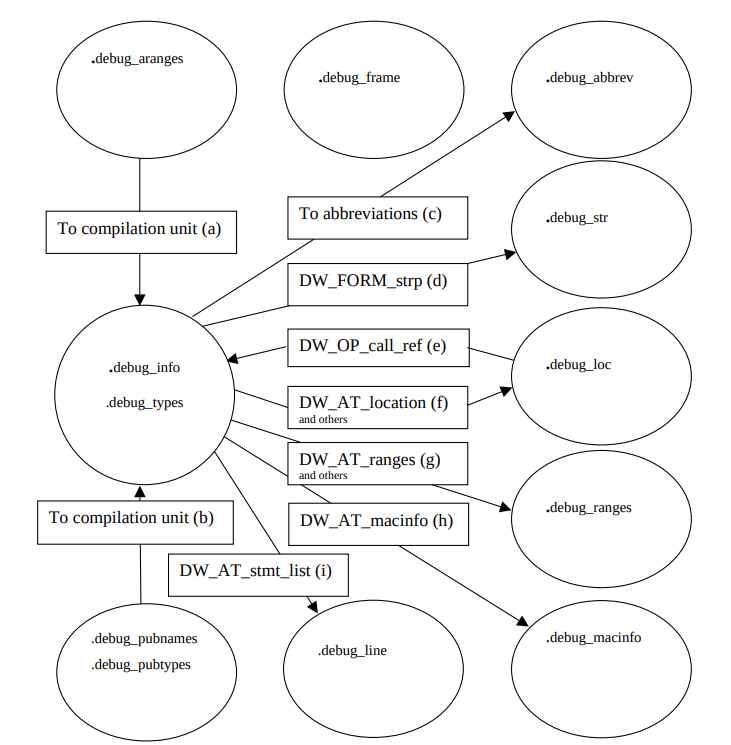
\includegraphics[width=1.0\textwidth]{dwarf-sections.png}
    \label{fig:dwarfsections}
\end{figure}


Going in alphabetical order the first \emph{DWARF} section is called \emph{.debug\_abbrev}.
This section contain all of the abbreviation tables which can be used to find a specific die using the abbreviation.
These table entries contain information about the die tag, attributes and if it has children.
The library \emph{gimli-rs} simplifies the process of using this table and thus removes the need to know the detail of how to read it, but checkout section 7.5.3 in \cite{dwarf} to know more.


The \emph{DWARF} section \emph{\.debug\_aranges} is used to lookup which machine address corresponseds to which compilations unit.
This address information is stored in ranges where a compilation unit can have multiple ranges.
These ranges consists of a start address followed by lenght.
Thus to lookup the user only needs to check if the search addres is between the start addres and the start address plus the lengh.
To read more about this section checkout section 6.1.2 in \cite{dwarf}.



\emph{.debug\_frame}


\emph{.debug\_info}
\emph{.debug\_line}
\emph{.debug\_loc}
\emph{.debug\_macinfo}
\emph{.debug\_pubnames}
\emph{.debug\_pubtypes}
\emph{.debug\_ranges}
\emph{.debug\_str}
\emph{.debug\_type}


% TODO: Explain DWARF Unit
% TODO: Explain DWARF Die and Attributes
% TODO: Explain evaluation

